% 01-introducao.tex | 1 Introduction
% RESTAURADO DO ORIGINAL em 06/11/2026 (pedido do Heitor: "nao remover o que foi escrito").
% Fonte: ArtigoExemplo/Paper Training - 15 Nov 2025.pdf, secoes 1 (Introduction) e 2.1 a 2.5 (Literature
% Review). A Production nao tem secao propria de revisao: a revisao virou 1.1 a 1.5 (como no artigo B).
% Da versao JATM ficou so o que nao conflita com o original: a contribuicao em tres itens e a Fig. 1.
% Edicao: gramatica e concisao; nenhuma afirmacao, numero ou citacao do original foi retirado.
% Mudancas de forma: "§7.2" -> "clause 7.2" (preferencia do autor); "GE Aviation" -> "an engine
% manufacturer" (duplo-cego); anos corrigidos so nas referencias verificadas (Kirkpatrick 2006,
% Leveson 2012, Reason 1990, Phillips 2016).
% Citacoes em vermelho no PDF = referencias do original nao localizadas (refs.bib, naolocalizada).
% Revisao de estilo (06/11/2026): frases longas divididas, intensificadores retoricos trocados, siglas
% definidas na 1a ocorrencia, linguagem causal ajustada ao desenho (estudo de caso sem grupo de controle).
% Nenhuma afirmacao, numero ou citacao do original foi retirado.

\section{Introduction}
\label{sec:introduction}

Aviation safety and sustainability depend on effective maintenance. In 2008, 15\% of air accidents involved maintenance events, and in 57\% of these, deficiencies in the operator's maintenance operations, such as deficient technical documentation and deficient training of maintenance personnel, were contributing factors \parencite{IATA2009}\citepend{ANAC, 2018}. \todo{número corrigido pela fonte real: o original citava IATA (2021), mas os dados são do Safety Report 2008 (IATA, 2009), e os 57\% são deficiências da manutenção do operador em geral, não só de treinamento. ANAC (2018) não foi identificada} The implications extend beyond safety. These deficiencies also generate considerable resource waste: scrapped high-value components, energy-intensive rework and unnecessary fuel consumption, which directly undermine the cleaner production goals of the aviation industry \parencite{Chen2023}. As global air travel grows, maintenance organizations face growing pressure to balance operational efficiency with strict safety and sustainability standards. The tension is acute in aircraft engine maintenance, a resource-intensive process that requires flawlessly executed technical procedures. Yet most aviation maintenance providers lack validated methods to quantify training effectiveness while ensuring compliance with \AS{} and civil aviation authority (\CAA{}) regulations. The gap has a safety cost and a resource cost: when training fails, the consequences include preventable accidents as well as substantial economic and environmental costs from non-conforming parts and procedural errors. Kirkpatrick's four-level model (reaction, learning, behavior, results) is established in generic training contexts, but its application in high-stakes, regulated aviation maintenance remains understudied. Prior research has not (1)~integrated Kirkpatrick with \AS{} and \CAA{} requirements, (2)~demonstrated how continuous training improvement reduces maintenance-induced risks or (3)~framed human reliability training as a core strategy for waste prevention and resource efficiency in line with sustainable operations \parencite{YangPark2024}.

While prior studies document training's role in reducing errors \parencite{EASA2025}, empirical evidence remains limited on integrating evaluation frameworks with regulatory mandates such as \AS{} clause 7.2. \todo{fonte conferida no PDF: o Annual Safety Review 2025 da EASA não trata do efeito do treinamento sobre erros; trocar a citação por uma fonte que trate} This creates a practical gap in which organizations prioritize compliance documentation over verifiable improvements, leading to persistent risks and waste. Training sits low in the hierarchy of risk controls, yet it interacts with socio-technical factors that explain a substantial share of post-training variance \parencite{OConnor2024}. The scientific value of this study lies in a synthesis: Kirkpatrick's model is operationalized as a continuous improvement mechanism for resource efficiency and human capital development \parencite{Sousa2025}, beyond its usual role in assessment, and validated in a real \AS{}-certified setting. The study addresses these gaps with a mixed-methods case study at a multinational aircraft engine maintenance facility. There, the authors developed and implemented an \AS{}-aligned Kirkpatrick framework and collected multi-source data to quantify its effects on quality and sustainability metrics. The study answers four research questions (RQs):

\begin{description}
  \item[RQ1.] What are the \AS{} and civil aviation regulation (CAR) training requirements?
  \item[RQ2.] How can the aircraft engine maintenance training management process be optimized by integrating reaction, learning, behavior and results evaluations?
  \item[RQ3.] How can Kirkpatrick's model be operationalized as a continuous improvement tool within \AS{} and \CAA{} constraints?
  \item[RQ4.] What is the impact of ineffective training on costs of quality and associated resource waste?
\end{description}

This work shows how aviation maintenance providers can embed Kirkpatrick's levels into routine training management and turn compliance exercises into strategic assets for safety and sustainability. Doing so reduces human-factor risks and material waste while meeting regulatory mandates. The study provides an empirically grounded blueprint for using training evaluation as a proactive tool for accident prevention and cleaner production in safety-critical aviation environments. The contribution is threefold: (a)~a mapping of Kirkpatrick's four levels to \AS{} clauses, Safety Management System (\SMS{}) components and sustainability indicators (Figure~\ref{fig:conceptual}); (b)~twelve months of operational evidence from an \AS{}-certified engine maintenance facility; and (c)~managerial and policy implications for maintenance, repair and overhaul (\MRO{}) managers, airline quality departments and aviation regulators. Sections 1.1 to 1.6 review the literature, state the research gaps and present the case context; Sections~\ref{sec:methods} to \ref{sec:conclusions} report the method, results, discussion and conclusions.

\begin{figure}[H]
  \centering
  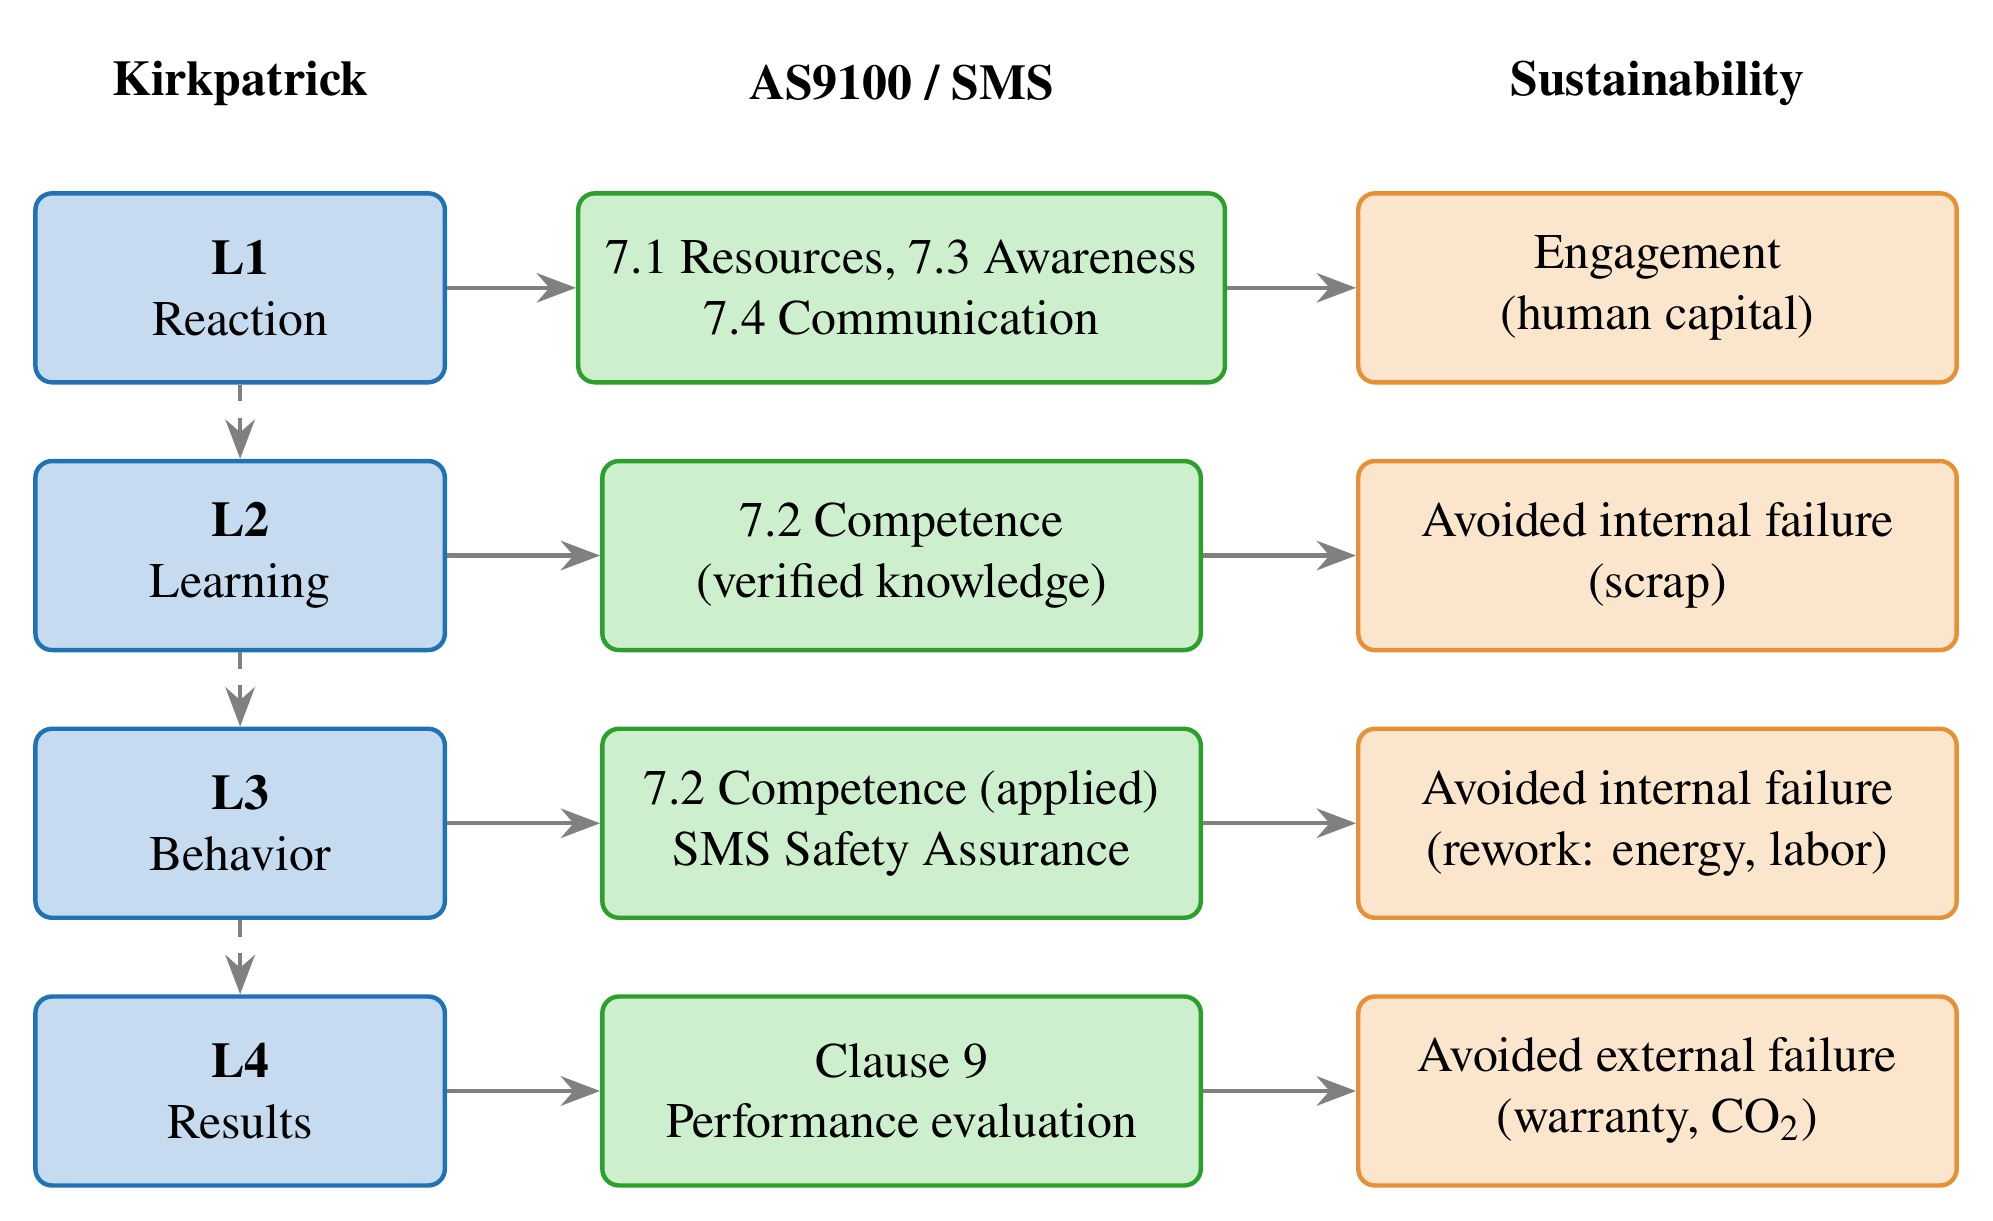
\includegraphics[width=0.9\linewidth]{fig1-conceptual-model}
  \caption{Conceptual model linking Kirkpatrick's four levels to AS9100 clauses, SMS components and sustainability outcomes}
  \label{fig:conceptual}
  \notafonte{Vertical dashed arrows represent the progression of the Kirkpatrick model; horizontal arrows represent the mapping proposed in this study. AS9100: aerospace quality management standard; SMS: Safety Management System. Source: the authors.}
\end{figure}

\subsection{Kirkpatrick's model: theoretical evolution and modern critiques}
\label{subsec:kirkpatrick}

Kirkpatrick's four-level framework \parencite{Kirkpatrick2006} evaluates participants' reaction, the knowledge or skill they acquire, the transfer of learning to job behavior and the organizational results. It remains foundational but faces mounting scrutiny in complex systems. Persistent limitations include its inability to isolate training effects from organizational variables at Level~4 \parencite{Patel2023}, cultural bias in Level~3 assessments \parencite{OConnor2024} and overreliance on self-reported data \parencite{KimLee2024}. Emerging solutions target these gaps. Artificial intelligence (AI)-enhanced attribution modeling using SHAP (SHapley Additive exPlanations) values quantifies training's contribution to outcomes \parencite{FernandezDelgado2024}; blockchain-verified competency tracking provides immutable Level~3 evidence \parencite{BoeingMRO2025}; and neuroergonomic assessments, such as electroencephalography (EEG) and functional near-infrared spectroscopy (fNIRS), replace satisfaction surveys at Level~1 \parencite{NASAHFB2023}. A theoretical gap persists, as no study has validated Kirkpatrick's model in \AS{}-regulated aviation environments \parencite{OReilly2024}. To enhance methodological rigor, this study employs advanced attribution techniques, such as SHAP values in regression models, to isolate training effects from confounders like shift length or supply chain variability, addressing Kirkpatrick's historical isolation challenges \parencite{FernandezDelgado2024}. \todo{o original diz que o estudo usa SHAP, mas a metodologia (seção 2) não descreve essa análise: incluir a análise ou reescrever como direção futura} This builds on production and operations management literature that emphasizes rigorous, data-driven solutions in operations, such as the optimization models for resource allocation in high-stakes environments of \textcite{Jung2019}. Future research directions include longitudinal studies integrating neuroergonomics (e.g., EEG at Level~1) to predict behavioral transfer, offering scalable tools for other regulated industries beyond aviation.

\subsection{Aviation maintenance training: regulatory imperatives and empirical shortfalls}
\label{subsec:aviation-training}

In aviation safety, maintenance errors drive 12--18\% of fatal accidents, with training deficiencies implicated in 73\% of cases \parencite{EASA2025}. \todo{fonte conferida no PDF (158 p.): o Annual Safety Review 2025 da EASA não traz 12--18\% nem 73\%; achar a fonte real dos números ou retirá-los (decisão dos autores)} The economic impacts are severe: engine test-cell rejections average USD~47,200 per incident \parencite{IATAMRO2025}, training-related warranty claims cost USD~189,500 each \parencite{Zhang2025}, and regulatory non-compliance penalties reach USD~2.1 million annually \parencite{FAA2024}. \todo{a AC 120-92D da FAA não traz valor de multa; o valor de USD 189.500 aparece na seção 1.5 como dado interno da empresa} Regulatory--operational misalignment exacerbates these issues: while \AS{} Rev~E (2024) mandates ``data-driven competency proof'', fewer than 35\% of repair stations comply \parencite{SAE2025}. \todo{a edição vigente em 2025 era a AS9100D (2016); conferir a existência da Rev E} \SMS{} pillars require training--safety integration but leave the method of evaluating training to each organization \parencite{Leveson2012,FAA2024}, creating a ``compliance paradox'' in which training hours do not equate to competency \parencite{Nakamura2024}.

\subsection{Human factors and socio-technical systems}
\label{subsec:human-factors}

Cognitive factors strongly influence maintenance errors: 72\% of procedural deviations stem from confirmation bias and normalization of deviance \parencite{Reason1990,Dismukes2023}. \todo{Reason (1990) sem PDF: o termo normalization of deviance é de Vaughan (1996), posterior ao livro, e o 72\% dificilmente está nele; conferir} Virtual reality training reduces spatial memory errors by 41\% compared with traditional methods \parencite{Airbus2024}. Organizational culture mediates outcomes, with safety culture maturity explaining 68\% of the variance in Level~3 knowledge transfer \parencite{OConnor2024}. High-reliability organizations exhibit two traits: just-culture reporting correlates strongly with training efficacy ($r = .79$), and leader-led safety dialogs occur five or more times a month \parencite{FAAHERMIT2024}. In system-safety terms, errors are properties of socio-technical systems as much as of individuals: \textcite{Reason2016} describes how latent and active failures combine, and systems-theoretic approaches emphasize hierarchical control and feedback \parencite{Leveson2012}. Two consequences follow for this study. A Level~2 (learning) outcome does not guarantee a Level~3 (behavior) outcome, because attention, fatigue, time pressure and supervision intervene. The data design must therefore combine post-training assessment with evidence from the workplace.

\subsection{Technological enablers for next-generation evaluation}
\label{subsec:tech-enablers}

Digital integration frameworks now connect Kirkpatrick's levels through continuous data flow: augmented reality feedback at Level~1, AI-proctored assessments at Level~2, Internet of Things (IoT)-enabled behavior tracking at Level~3 and causal machine-learning analytics at Level~4. Real-world implementations report measurable effects: an engine manufacturer's digital twin simulations reduced CFM56 engine misassembly by 33\% \parencite{Garcia2024}, and Lufthansa Technik's blockchain credentials cut audit time by 62\% \parencite{IATABlockchain2025}. In predictive analytics, convolutional neural networks forecast training return on investment (\ROI{}) with 89\% accuracy \parencite{Peterson2025}, and natural language processing of maintenance logs detects latent skill gaps \parencite{BoeingAIR2024}. \todo{o original cita a empresa pelo nome no exemplo do gêmeo digital; trocado por "an engine manufacturer" para a revisão cega}

\subsection{Research gaps}
\label{subsec:gaps}

Existing literature establishes Kirkpatrick's model as a well-tested framework for training evaluation across general industries \parencite{Phillips2016,BuriakAyars2019}, yet the model shows important limitations in safety-critical aviation contexts. While foundational studies validate the four-level structure conceptually, they neglect the regulatory constraints of \AS{}-certified environments \parencite{OReilly2024}. Three gaps follow. First, prior works treat compliance and evaluation as parallel concerns rather than integrated requirements, addressing either Kirkpatrick's generic implementation \parencite{Kirkpatrick2006} or quality management requirements, such as the implementation of \AS{} and its documentation clauses \parencite{YucelAyvaz2019} and total quality management \parencite{Oschman2017}, in isolation. No existing methodology maps the reaction--learning--behavior--results progression to the competency evidence required by \AS{} clause 7.2, and this disconnect between regulation and practice undermines audit readiness. \todo{fontes ajustadas: Oschman (2017) trata de TQM (resumo conferido, sem PDF); Yücel \& Ayvaz (2019), que estava na lista do original sem ser citada, trata da implantação da AS9100 (página da editora conferida); conferir nos PDFs} Second, researchers acknowledge aviation's high-stakes economics \parencite{Zhang2025} but do not quantify training's causal relationship with safety-critical key performance indicators. Studies rank quality-management-system risks and their effects on organizational sustainability \parencite{Pereira2017} or attribute accidents statistically to categories of maintenance deficiency, although accident records lack performance-shaping factors \parencite{Boyd2015}; such studies do not isolate training's contribution from confounders such as supply chain delays or tooling failures. \todo{frase ajustada ao que as fontes dizem: Boyd \& Stolzer (2015) conferido no PDF; Pereira et al. (2017) pelo resumo, sem PDF: o autor correspondente confirma} Third, the predictive potential of Kirkpatrick data remains underexplored: AI-driven models forecast generic training \ROI{} \parencite{Peterson2025} but lack aviation maintenance specificity and ignore failure-cost preemption. The framework proposed here uses Level~1--3 analytics to redirect resources toward high-risk competencies, moving evaluation from retrospective accounting, such as warranty claim analysis \parencite{Zhang2025}, to prospective risk mitigation. Theoretical limitations also persist. Cultural and technological barriers receive nominal acknowledgement \parencite{OConnor2024} but no operational path to resolution. Studies that identify the compliance paradox \parencite{Nakamura2024} offer no blueprint for resolving the mismatch between training hours and competency that affects \MRO{} organizations, and emerging technologies such as blockchain credentialing \parencite{IATABlockchain2025} remain unvalidated in legacy aviation quality systems. This study confronts these implementation challenges through workflow-embedded assessment protocols synchronized with \SMS{} reporting cycles and enterprise resource planning (\ERP{}) data. It bridges three domains that have remained separate (Kirkpatrick's evaluation theory, the regulatory architecture of \AS{} and the safety-economic realities of aviation) and converts training data into auditable safety assurance. This matters because 73\% of maintenance-related accidents involve evaluable training deficiencies \parencite{EASA2025}. \todo{o 73\% não está no relatório da EASA (PDF conferido)}

\subsection{Bridging theory to practice: economic impacts, guidelines and applicability}
\label{subsec:bridge}

This study documents a real-world problem at a multinational \MRO{} facility: recurrent training failures leading to warranty claims of USD~189,500 per incident and 35\% non-compliance in \AS{} audits (internal data, 2024). \todo{este 35\% é linha de base (auditorias AS9100, 2024); no resumo e nos Resultados, 35\% é a redução das constatações da autoridade por ciclo de auditoria (seção 2.2). Confirmar se são duas medidas diferentes e dar a unidade de cada uma} The company's previous solution, ad hoc post-incident retraining, lacked systematic evaluation and left gaps such as procedural deviations unaddressed (73\% of errors according to \cite{EASA2025}). \todo{idem: o 73\% não está no relatório da EASA} The approach adopted here integrates Kirkpatrick with \AS{} workflows in a replicable methodology: (1)~map training to risk hierarchies; (2)~use multi-source data (for example, \LMS{} records and observations) for Levels 1--4; and (3)~apply causal analytics to quantify \ROI{}. \todo{o método (seção 2) não descreve análise causal, observação no posto de trabalho nem o mapeamento para hierarquias de risco: descrever no método ou reescrever estas etapas como intenção} Over twelve months of implementation, the facility recorded about USD~1.2 million in annual savings, associated with a 28\% reduction in training failures. Discussions with facility managers revealed strong buy-in: ``This shifted us from reactive compliance to proactive risk mitigation'' (anonymous manager interview, 2025). Guidelines for practitioners include starting with a baseline audit of current training against \AS{} clause 7.2, piloting Level~3 assessment in high-risk modules and scaling through \ERP{} integration. The approach can be transferred to other sectors, such as automotive or healthcare organizations under ISO 9001. It also opens production and operations management directions, such as hybrid AI--human models for predictive training in global operations, extending behavioral operations evidence that human servers do not behave like machines \parencite{Shunko2018}.
